\documentclass[12pt, twoside]{article}
\usepackage[letterpaper, margin=1in, headsep=0.5in]{geometry}
\usepackage[english]{babel}
\usepackage[utf8]{inputenc}
\usepackage{amsmath}
\usepackage{amsfonts}
\usepackage{amssymb}
\usepackage{tikz}
\usetikzlibrary{quotes, angles}
\usepackage{graphicx}
\usepackage{enumitem}
\usepackage{multicol}

\newif\ifmeta
\metatrue %print standards and topics tags

\title{IB Math Applications and Interpretations}
\author{Chris Huson}
\date{March 2022}

\usepackage{fancyhdr}
\pagestyle{fancy}
\fancyhf{}
\renewcommand{\headrulewidth}{0pt} % disable the underline of the header
\raggedbottom

\fancyhead[LE]{\thepage}
\fancyhead[RO]{\thepage \\ Name: \hspace{4cm} \,\\}
\fancyhead[LO]{BECA / IB Math 6 Geometry \\* 29 March 2022}

\begin{document}
\subsubsection*{6.6 Pre-Quiz: Non-right triangle trigonometry \hfill HSG.SRT.D.11}
\emph{Round all values to three significant figures.}
\begin{enumerate}
\item Do Now: Given right $\triangle ABC$ with $AB=10$, $m\angle A=53^\circ$. Find the value of $BC=x$.
  \begin{flushright}
    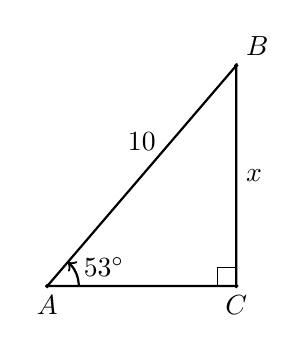
\begin{tikzpicture}[scale=0.4]
      \draw [thick](0,0)--(6,0)--(6,7)--cycle;
      \draw [fill] (0,0) circle [radius=0.05] node[below]{$A$};
      \draw [fill] (6,0) circle [radius=0.05] node[below]{$C$};
      \draw [fill] (6,7) circle [radius=0.05] node[above right]{$B$};
      \draw (6,0)++(-0.6,0)--++(0,0.6)--+(0.6,0);
      \node at (3,4)[above]{$10$};
      \node at (6,3.5)[right]{$x$};
      \draw [thick, ->] (1,0) arc [start angle=0, end angle=49, radius=1];
      \node at (1.8,0)[above]{$53^\circ$};
    \end{tikzpicture}
  \end{flushright}

\subsubsection*{Area of a triangle sine formula \hfill HSG.SRT.D.9}  
\item Given $\triangle ABC$ with $AC=12$ centimeters, base $AB=16$, and the base $\hat{A} = 55^\circ$. (diagram not to scale)
\begin{multicols}{2}
  \begin{enumerate}
    \item Find altitude $h$ cm using $\displaystyle \sin \hat{A}=\frac{h}{12}$.
    \item Find the area of the triangle\\[0.5cm]
    $Area = \frac{1}{2}bh$
  \end{enumerate}
  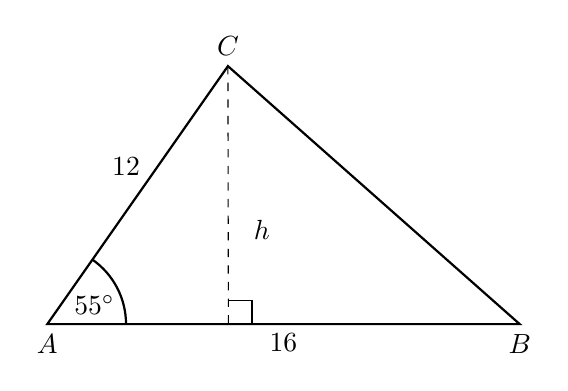
\begin{tikzpicture}[scale=1]
    \draw [thick]
      (0,0)node[below]{$A$}--
      (6,0)node[below]{$B$}--
      (55:4)node[above]{$C$} --cycle;
    \draw [dashed] (55:4)--(2.3,0);
    \draw (2.3,0)++(0.3,0)--++(0,0.3)--+(-0.3,0);
    \node at (2.5,1.2)[right]{$h$};
    \node at (1,2){$12$};
    \node at (3,0)[below]{$16$};
    \draw [thick, -] (1,0) arc [start angle=0, end angle=55, radius=1];
    \node at (0.6,0)[above]{$55^\circ$};
    %\node at (5,0)[below]{$13 \frac{1}{2}$ cm};
  \end{tikzpicture}  
\end{multicols}
\vspace{1cm}

\item Find the area of the given triangle. Triangle area using sine formula: $A=\frac{1}{2}ab \sin C$
\begin{flushright}
  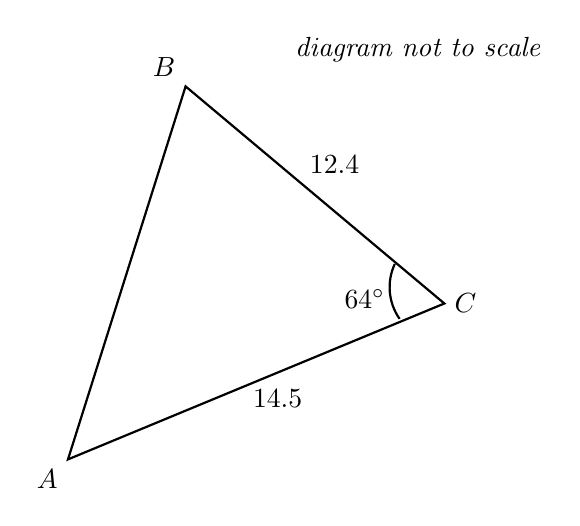
\begin{tikzpicture}[scale=0.7]
    \draw [thick](0:4)node[right]{$C$}--
    (100:4)node[above left]{$B$}--
    (-135:4)node[below left]{$A$}--cycle;
    \node at (55:3.5)[below]{$12.4$};
    \node at (-55:1.7)[below]{$14.5$};
    \draw [thick, -] (-5:3.2) arc [start angle=215, end angle=155, radius=1];
    \node at (1.5:3.1)[left]{$64^\circ$};
    \node at (50:5.5)[above]{\emph{diagram not to scale}};
  \end{tikzpicture}
\end{flushright}

\newpage
\subsubsection*{The sine rule \hfill HSG.SRT.D.11}
$\displaystyle \frac{a}{\sin A} = \frac{b}{\sin B} = \frac{c}{\sin C}$
\item The following diagram shows triangle $ABC$, with $A\hat{B}C=40^\circ$, $A\hat{C}B=35^\circ$, and $AC=10.6$ cm. \\[0.25cm]
Find $AB$. \hfill \emph{diagram not to scale}
  \begin{flushright}
    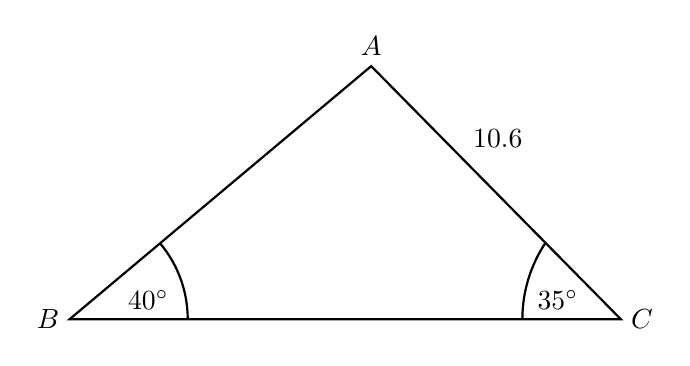
\begin{tikzpicture}[scale=1]
      \draw [thick](40:5)node[above]{$A$}--
      (0,0)node[left]{$B$}--
      (0:7)node[right]{$C$}--cycle;
      \node at (25:6)[below]{$10.6$};
      \draw [thick, -] (0:1.5) arc [start angle=0, end angle=40, radius=1.5];
      \node at (0:1)[above]{$40^\circ$};
      \draw [thick, -] (0:5.75) arc [start angle=180, end angle=146, radius=1.75];
      \node at (0:6.2)[above]{$35^\circ$};
    \end{tikzpicture}
  \end{flushright}\vspace{2cm}

\item Triangle $ABC$ is drawn with $AC=102$ cm, $BC=86$ cm, and $A\hat{B}C=71^\circ$. \\[0.25cm]
Find $B\hat{A}C$.
  \begin{flushright}
    \begin{tikzpicture}[scale=0.8, rotate=-40]
      \draw [thick](0:4)node[right]{$B$}--
      (100:4)node[above right]{$C$}--
      (-135:4)node[below left]{$A$}--cycle;
      \node at (55:3.2)[below]{$86$};
      \node at (150:2.75)[below]{$102$};
      \draw [thick, -] (-5:3.2) arc [start angle=215, end angle=155, radius=1];
      \node at (1.5:2.8)[above]{$71^\circ$};
      \node at (100:5.5)[above]{\emph{diagram not to scale}};
    \end{tikzpicture}
  \end{flushright}
  
\newpage
\subsubsection*{The cosine rule \hfill HSG.SRT.D.11}
$c^2 = a^2+b^2- 2ab \cos C$
\item As shown in the diagram, triangle $ABC$ has $A\hat{B}C=47^\circ$, $AB=7.3$, and $BC=15.2$. \\[0.25cm]
Find $AC$. \hfill \emph{diagram not to scale}
  \begin{flushright}
    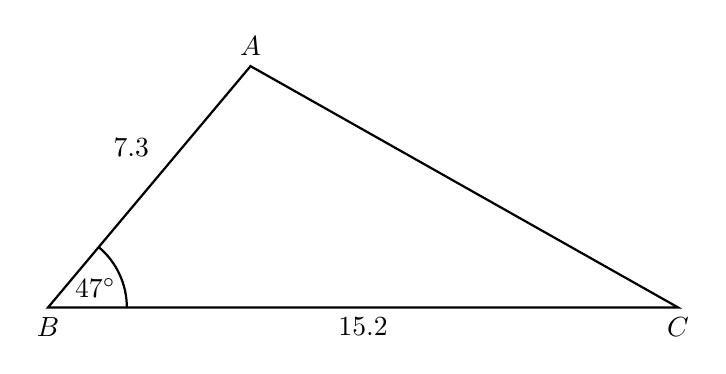
\begin{tikzpicture}[scale=1]
      \draw [thick](50:4)node[above]{$A$}--
      (0,0)node[below]{$B$}--
      (0:8)node[below]{$C$}--cycle;
      \node at (65:2.5)[below]{$7.3$};
      \node at (0:4)[below]{$15.2$};
      \draw [thick, -] (0:1) arc [start angle=0, end angle=50, radius=1];
      \node at (0:0.6)[above]{$47^\circ$};
    \end{tikzpicture}
  \end{flushright}\vspace{1cm}

\item The following diagram shows triangle $PQR$. (\emph{not to scale}) \\[0.25cm]
$PQ=17$ meters, $QR=23$ m., and $PR=12$ m. \\[0.25cm]
Find $P\hat{Q}R$.
  \begin{flushright}
    \begin{tikzpicture}[scale=1, rotate=20]
      \draw [thick](60:6.5)node[above]{$Q$}--
      (0,0)node[left]{$P$}--
      (-45:4.6)node[below]{$R$}--cycle;
      \node at (70:3.5)[below]{$17$};
      \node at (-50:2.25)[below]{$12$};
      \node at (20:4)[below]{$23$};
    \end{tikzpicture}
  \end{flushright}

\newpage
\item A ladder that is 4 meters long leans against a wall making an angle to the ground of $68^\circ$, as shown in the diagram.  \hfill (not drawn to scale)
  \begin{multicols}{2}
    \begin{enumerate}
      \item Find the height of the top of the ladder above the ground. \vspace{2cm}
      \item Find the distance of the bottom of the ladder to the base of the wall.
    \end{enumerate} 
    \begin{flushright}
    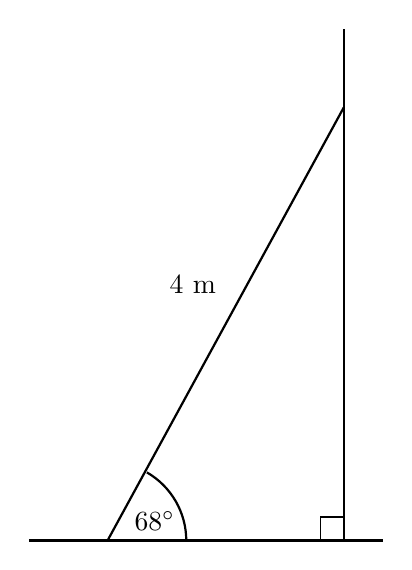
\begin{tikzpicture}[scale=0.5]
      \draw [thick](0,0)--(9,0);
      \draw [thick](8,0)--(8,13);
      \draw [thick](2,0)--(8,11);
      \draw (8,0)++(-0.6,0)--++(0,0.6)--+(0.6,0);
      \node at (5,6.5)[left]{$4$ m};
      \draw [thick, -] (0:4) arc [start angle=0, end angle=60, radius=2];
      \node at (0:3.2)[above]{$68^\circ$};
    \end{tikzpicture}
    \end{flushright}
  \end{multicols}
  \vspace{3cm}

\item The following diagram shows a triangle $ABC$. \hfill (diagram not to scale)\\[0.5cm]
The area of the triangle $ABC$ is 80 $\rm{cm}^2$, $AB=18$ cm, $AC=x$ cm, and $B\hat{A}C = 50^\circ$.
  \begin{multicols}{2}
    \begin{enumerate}
      \item Find $x$.
      \item Find $BC$.
    \end{enumerate}
    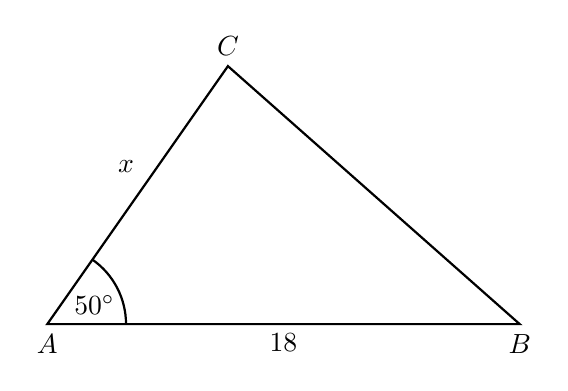
\begin{tikzpicture}[scale=1]
      \draw [thick]
        (0,0)node[below]{$A$}--
        (6,0)node[below]{$B$}--
        (55:4)node[above]{$C$} --cycle;
      \node at (1,2){$x$};
      \node at (3,0)[below]{$18$};
      \draw [thick, -] (1,0) arc [start angle=0, end angle=55, radius=1];
      \node at (0.6,0)[above]{$50^\circ$};
      %\node at (5,0)[below]{$13 \frac{1}{2}$ cm};
    \end{tikzpicture}  
  \end{multicols}
  \vspace{1cm}

\end{enumerate}
\end{document}
